\chapter{NVidia GPU指令集架构-程序控制和原子操作}

\begin{center}\small 作者：reed（知乎 @reed-84-49，专栏「CUDA高性能编程」）\quad 原文：\url{https://zhuanlan.zhihu.com/p/712357443}\end{center}

在前面的文章中，我们详细介绍了NVIDIA GPU中的浮点计算(\url{https://zhuanlan.zhihu.com/p/695667044})、整数计算(\url{https://zhuanlan.zhihu.com/p/700921948})、位操作(\url{https://zhuanlan.zhihu.com/p/712356884})以及Warp级协同计算(\url{https://zhuanlan.zhihu.com/p/712357647})，这些构成了GPU的核心计算能力，为图形渲染和AI计算提供了强大的支持。此外，我们还探讨了GPU的寄存器(\url{https://zhuanlan.zhihu.com/p/688616037})、加载/存储单元和缓存机制(\url{https://zhuanlan.zhihu.com/p/692445145})，它们负责数据的存储和传输，确保计算单元能够高效地获取和处理数据。

然而，计算和数据搬运只是GPU功能的一部分，程序控制逻辑同样是不可或缺的。程序控制逻辑负责协调计算流程，确保程序按照预期的逻辑执行。尽管GPU是一个高度并行的系统，但在许多情况下，我们仍然需要局部或全局的串行逻辑来完成程序控制和数据同步。为此NVIDIA GPU提供了一系列原子操作指令，以支持这些需求。

本文将重点介绍NVIDIA GPU的程序控制逻辑和原子操作指令。首先，我们将从编程语言层和底层指令的对应逻辑开始介绍，逐步深入到指令层的控制流，探讨Predicate、SEL、BRA等指令在程序控制中的作用，然后我们介绍了原子指令ATOM、ATOMG、ATOMS以及更高效的RED指令，最后文章对全文进行了总结。

\section{高级编程语言和底层指令}

在高级编程语言（如CUDA C）中，控制流结构, 如if、for、while、switch、goto、function call、return被广泛使用（如图1），这些结构可以为高级编程语言提供丰富的控制和表达能力，底层硬件指令在实现时会结合GPU多线程、高并行的硬件特征提供更底层和原子的控制能力。具体地，NVidia GPU提供了Predicate能力，Select、Branch、Call、Return、Exit等相关指令来完成程序控制（如图1所示）。

\begin{figure}[htbp]\centering
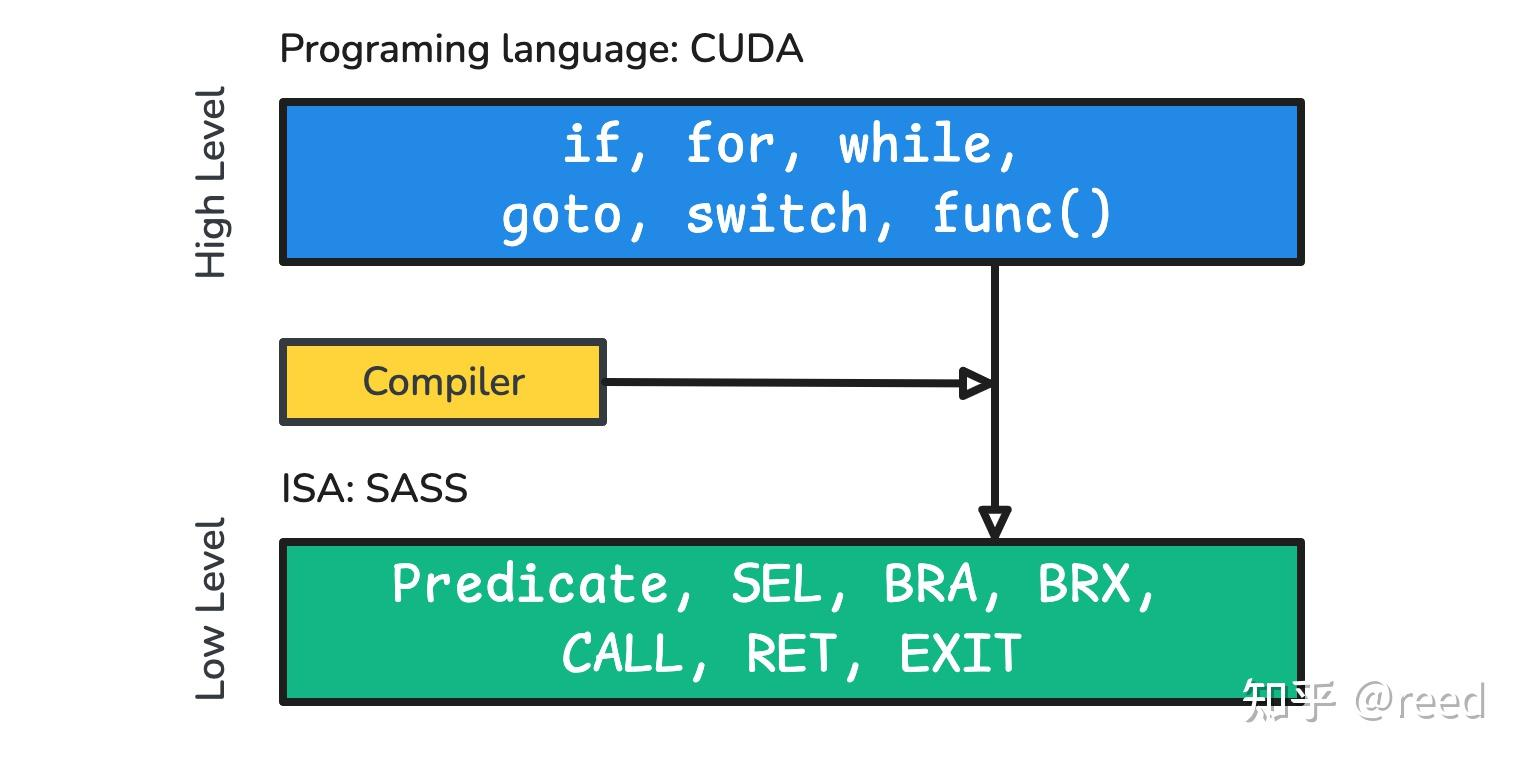
\includegraphics[width=0.9\textwidth]{figures/reed-isa-08-control-atomics/fig-01.jpg}
\caption{Figure 1. High level CUDA and Low Level SASS}
\end{figure}

利用或组合这些指令可以表达出高层语言的控制流结构。值得注意的是，高层语言和底层指令并不是一一对应，同一个高层语言的逻辑可以对应底层指令的多种组合形式，如有些if逻辑可以通过Predicate实现，可以通过SEL实现，也可以通过BRA实现，但是针对不同的场景效率会有很大的差别，编译器会结合具体的上下文给出更好的指令选择。

\section{指令层的控制流}

Predicate实现控制流

如下CUDA代码展示了if 控制流，在lower到指令集时，一般会使用Predicate来完成控制，

\begin{lstlisting}
  if (c > 0) {
    v = __sinf(f);
  } else {
    v = __cosf(f);
  }
\end{lstlisting}

上述CUDA代码对应的指令表示

\begin{lstlisting}
@!P0 MUFU.COS R0, R8 ;
@P0 MUFU.SIN R0, R8 ;
\end{lstlisting}

从上面可以看到高层编程语言的if控制流在底层指令中是通过Predicate来实现。

选择指令（SEL）

CUDA编程语言中的if语句，如果满足某种约定且足够简单，则编译器可以从后端的指令集中选择SELect指令，如下CUDA语句

\begin{lstlisting}
  if (c > 0) {
    v = 1;
  } else {
    v = 2;
  }
\end{lstlisting}

则编译器生成指令的一种可能的行为如下：

\begin{lstlisting}
MOV R7, 0x1 ;
...
SEL R7, R7, 0x2, P0 ;
\end{lstlisting}

其中P0为Predicate寄存器，其表达了\lstinline|c > 0| 这个条件，如果条件成立，则选择R7, 否则选择立即数 0x2 (即整数2)。SEL指令在SIMIT意义下可以避免跳转的开销，提升执行效率。

分支指令（BRA，BRX，BRXU）

branch分支指令可以实现指令的跳转，如CUDA代码中的for循环，

\begin{lstlisting}
  float v = 0.f;
#pragma unroll 1
  for (int i = 0; i < n; ++i) {
    v += ff;
  }
\end{lstlisting}

则可以通过分支跳转指令实现，一种可能的指令序列如下

\begin{lstlisting}
/*0070*/                   IADD3 R3, R3, 0x1, RZ ;
/*0080*/                   FADD R0, R0, c[0x0][0x184] ;
/*0090*/                   ISETP.GE.AND P0, PT, R3, c[0x0][0x180], PT ;
/*00a0*/              @!P0 BRA 0x70 ;
\end{lstlisting}

其中IADD 语句表示整数加一，对应于CUDA中的i++; FADD语句表示浮点加法，对应于CUDA中的\lstinline|v += ff|;ISETP 语句表示根据整数比较结果来设置Predicate寄存器，其中比较的条件为GE(Greater than and Equal) ，对应于CUDAfor语句中的 \lstinline|i < n| 的取反条件表示。 \lstinline|@!P0 BRA 0x70 ;| 表示P0条件不成立时则跳转到0x70位置执行。通过BRA跳转语句实现了for的循环能力。

除了以上的给定地址的分支跳转，NVidia GPU指令集中还提提供了动态的跳转指令BRX，其指令实例为\lstinline|BRX R6 -0x7960|形式， 它根据寄存器的值进行更动态的分支跳转能力，在switch语句实现中有可能出现该指令。同时还提供了根据Warp Level的Uniform寄存器值进行动态跳转的指令BRXU，命令形式如 \lstinline|BRXU UR34 -0xb200|。

执行Uniform执行

函数调用和返回（CALL，RET）

在CUDA中可以通过\lstinline|__device__|定义device函数，这些device函数可以在global函数中进行调用，对于比较小的函数，编译器一般会对此类函数进行inline优化，使其成为主函数的一部分，减少函数调用的指令的使用，但是有时候依然会使用到函数调用指令，在NVidia GPU中，常见的函数调用指令如下，Modifier有REL/ABS和NOINC：

\begin{lstlisting}
CALL.REL 0x60f0;
CALL.REL.NOINC 0xfd00;
CALL.ABS.NOINC R2;
\end{lstlisting}

其中Modifier REL表示相对调用，ABS表示绝对调用，NOINC表示PC值不改变。函数返回常见的指令为

\begin{lstlisting}
RET.ABS R18 0x20;
RET.REL.NODEC R80 0x0;
\end{lstlisting}

由于NVidia并没有公开其函数调用的ABI约定，并且GPU是一个拥有大量寄存器的设备，其很难在调用时把大量的寄存器都save下来，并且大部分函数都在一个编译单元内部，其有很大的优化空间，并且这部分内容更多的是编译器约定的范畴，此处就不做过多解读。

线程退出（EXIT）

由于GPU是一个多线程设备，大部分情况下不同的线程会执行同样的指令，有些时候其中的某些线程并不需要工作，其可以提前退出，NVidia GPU也提供了相应的指令

\begin{lstlisting}
EXIT ;
\end{lstlisting}

执行了该指令的线程并不会因为同warp的线程没有退出而执行其它指令，但值得注意的是，虽然warp内的某些线程执行了EXIT指令但是如果warp中仍有active线程，那么这些线程在执行SYNC、BAR等指令时行为应当是正确的。和其他指令类似，该指令也是可以被Predicate的，如

\begin{lstlisting}
@P2 EXIT
\end{lstlisting}

执行逻辑分裂与合并

由于GPU是多线程模型，在某些场景下需要一部分线程执行一个基本块，另一部分线程执行另外的基本块，这样可以确保逻辑正确，但是长期分裂执行会导致效率低下，NVidia GPU提供了相应的指令来显式的设置同步点，以达到高效的目的，具体的有如下指令实例：

\begin{lstlisting}
BSSY B0, 0x150
BSYNC B0 ;
@!P0 BREAK B2 ;
\end{lstlisting}

其中BSSY表示设置同步点指令，BSYNC为同步等待指令，BREAK为打破同步点指令，这些指令对于处理复杂的嵌套条件有重要作用，同时NVidia并没有对用户开放这部分能力，这部分能力由编译器裁决，更详细的信息可以参考NVidia的专利(\url{https://patents.google.com/patent/US11847508B2})。

除此之外，NVidia GPU中常见的控制相关的指令还有NOP(No Operation)和LEPC(Load Effective PC)等指令：

\begin{lstlisting}
NOP;
LEPC R96;
\end{lstlisting}

\section{原子操作}

前面我们介绍的计算类指令逻辑上要么是单个线程独立工作，要么是Warp Level协同工作，它们具有很好的局部性和独立性。在一些应用中，除了各个线程独立的计算之外，还需要在Block上进行规约或者计数操作，并且这些操作要求在逻辑上是原子执行的，为此NVidia GPU指令集架构中引入了Atomic类指令，其主要包含

\begin{lstlisting}
ATOM, ATOMS, ATOMG, RED
\end{lstlisting}

其中ATOMS和ATOMG分别是在Shared Memory空间和Global Memory空间上进行原子操作，ATOM指令没有具体的地址空间限定为generic的原子操作，如果编译器可以显式的推断出地址空间则使用对应的指令，如果不能推断出地址空间则可以使用通用的指令，这时硬件在运行时裁决是哪一个地址空间。NVidia GPU通过Modifer来实现不同的运算的，如加，最小，异或、与、CAS等（具体支持的操作可以参考图二AtomicALU部分），也通过Modifier来实现不同的作用Scope。常用的指令形式有

\begin{lstlisting}
ATOMS.ADD  ATOMS.ARRIVE.64 ATOMS.MIN.S32 ATOMS.POPC.INC.32
ATOM.E.ADD.STRONG.GPU  ATOM.E.ADD.STRONG.SYS  ATOM.E.CAS.STRONG.GPU  ATOM.E.EXCH.STRONG.SYS
ATOMG.E.ADD.64.STRONG.GPU ATOMG.E.ADD.STRONG.SYS    ATOMG.E.CAS.STRONG.GPU
ATOMG.E.ADD.STRONG.GPU    ATOMG.E.CAS.64.STRONG.GPU ATOMG.E.EXCH.STRONG.SYS
\end{lstlisting}

具体的ATOM类指令的形式如下，其语义为将R9的值原子的加在全局地址空间[R4.64]上，并返回加之前的值，获取值和加是原子的不能被其它操作打断。

\begin{lstlisting}
ATOMG.E.ADD.STRONG.GPU PT R5 [R4.64] R9
\end{lstlisting}

有时候我们只需要原子操作并不需要返回值，NVidia GPU提供了更轻量的原子指令RED，如图2，

\begin{figure}[htbp]\centering
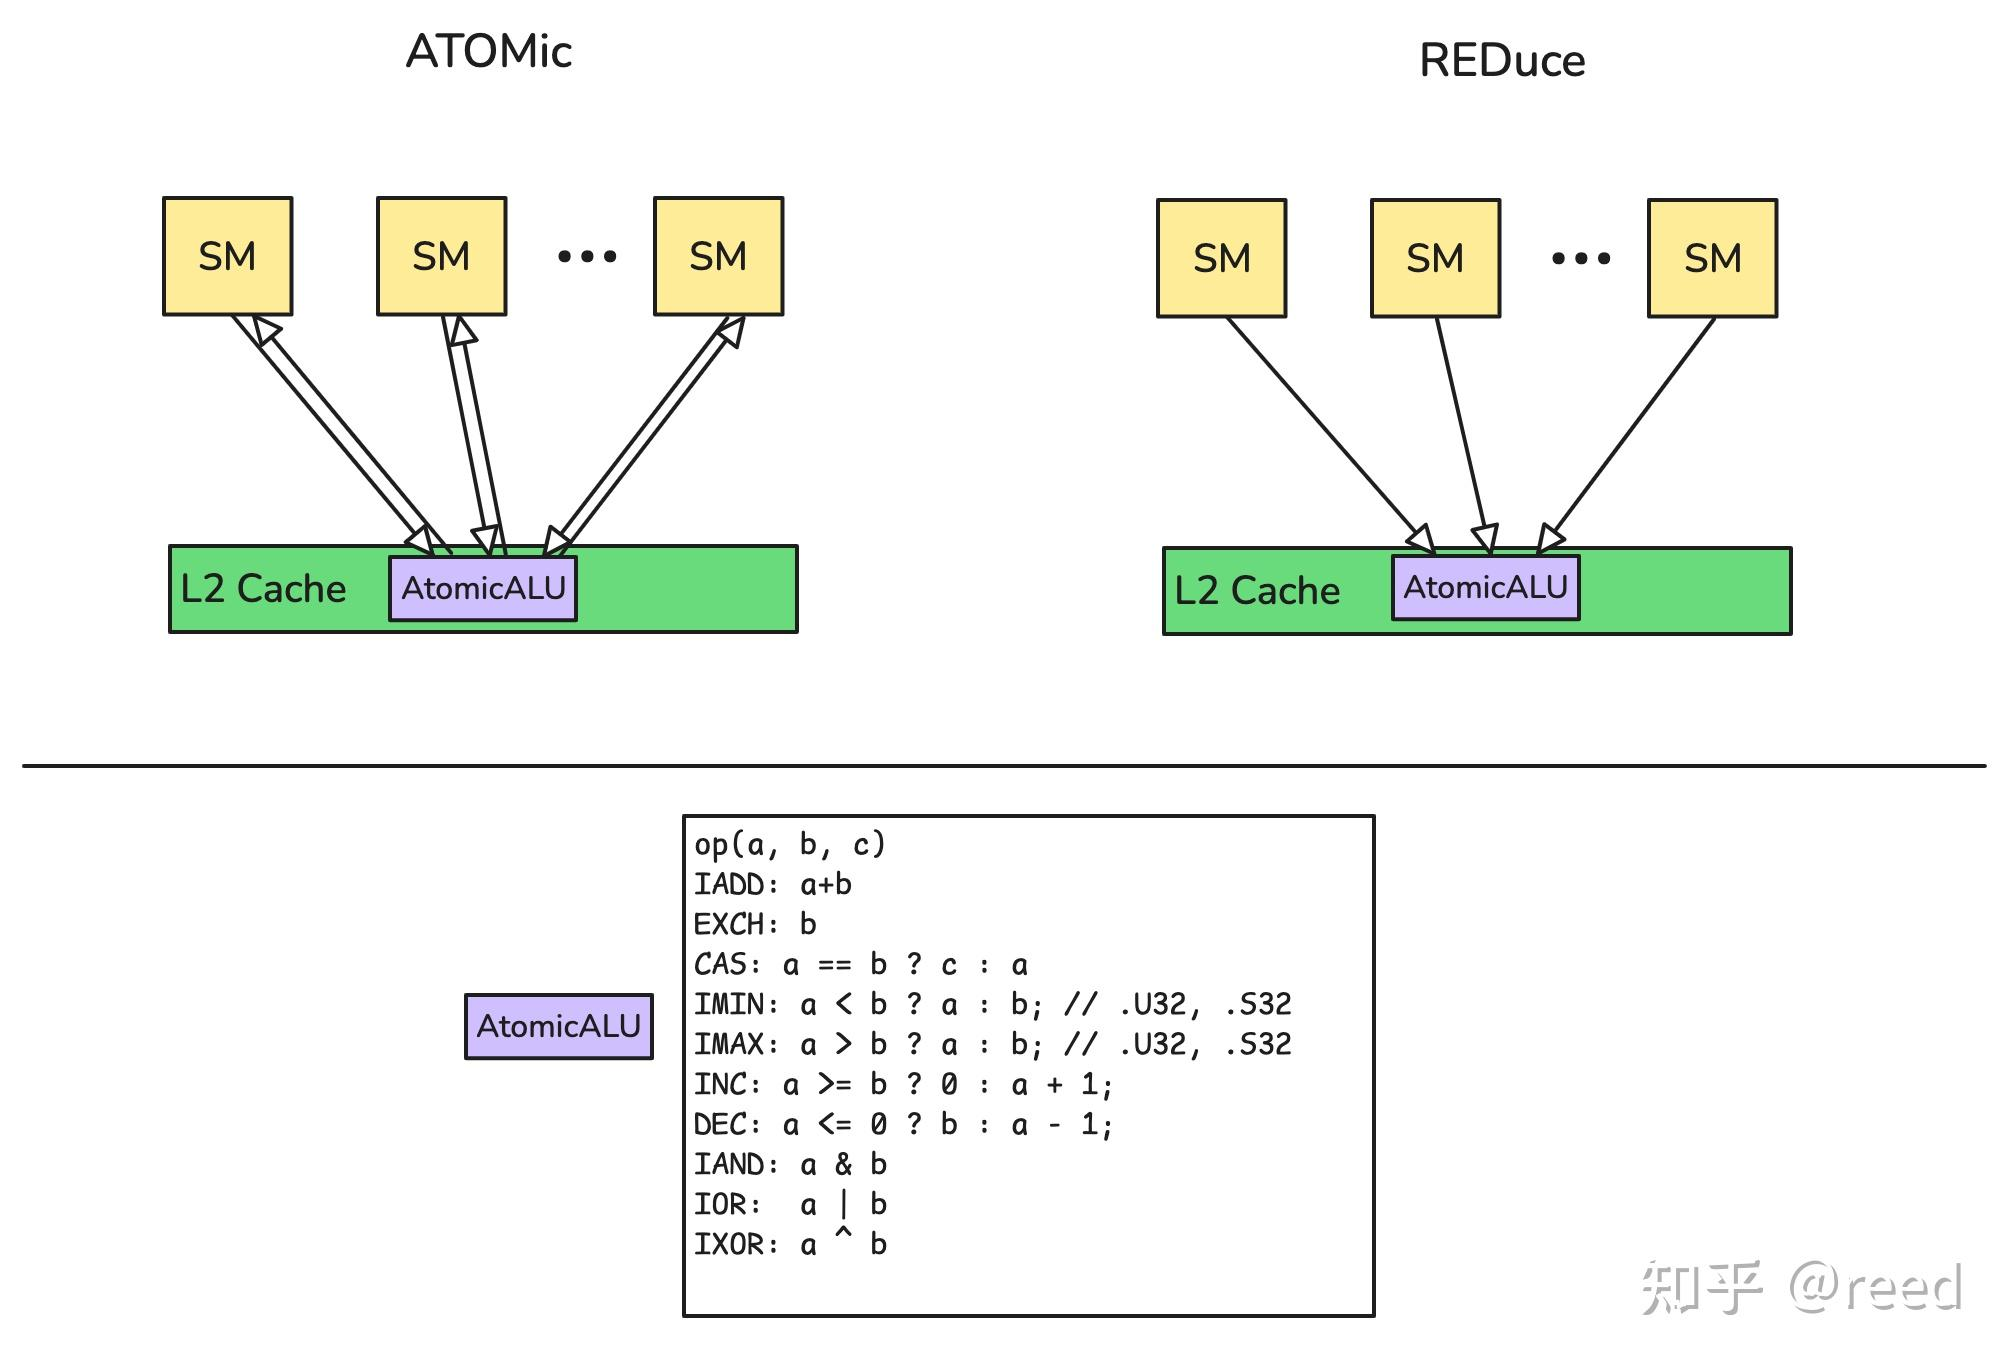
\includegraphics[width=0.9\textwidth]{figures/reed-isa-08-control-atomics/fig-02.jpg}
\caption{Figure 2. ATOM and RED Operation Difference and Supported Operation}
\end{figure}

ATOM指令需要获取读取的值，RED不需要。针对最终的内存而言，RED和ATOM的副作用一致。由于RED不必返回原子操作之前的值，效率也自然的会更高，具体的差异可以参看NVidia的专利(\url{https://patents.google.com/patent/US7627723B1})。

\begin{lstlisting}
RED.E.ADD.64.STRONG.GPU         RED.E.ADD.STRONG.GPU            RED.E.OR.STRONG.GPU
RED.E.ADD.F32.FTZ.RN.STRONG.GPU RED.E.MAX.S32.STRONG.GPU
RED.E.ADD.F64.RN.STRONG.GPU     RED.E.MIN.S32.STRONG.GPU
\end{lstlisting}

具体的指令形式为

\begin{lstlisting}
RED.E.MAX.S32.STRONG.GPU [R4.64] R7
\end{lstlisting}

从RED的指令形式我们可以看到其相较于ATOM指令，只需要输入数据的寄存器和操作的地址数据，并不会返回数据，从而也减少了返回数据的开销，提升了指令的效率。

\section{总结}

本文介绍了高级编程语言中的控制流和底层的程序控制的指令，指出了它们之间可能的多映射关系，针对不同的场景有不同的优化和映射方式，同时针对底层程序控制指令进行了详细介绍：Predicate实现控制流、SEL选择指令，BRA分支指令、函数调用CALL和返回RET指令，指出EXIT退出指令并不是简单的退出而需要考虑其他的BARRIER的一致性行为和并行执行引入的分裂和合并逻辑。同时文章介绍了原子指令，和无需返回值的RED类指令，了解这些指令能够更好的了解高并行硬件和相关编译器设计。

\section{参考}

reed：NVidia GPU指令集架构-浮点运算(\url{https://zhuanlan.zhihu.com/p/695667044})

reed：NVidia GPU指令集架构-整数运算(\url{https://zhuanlan.zhihu.com/p/700921948})

reed：NVidia GPU指令集架构-比特和逻辑操作(\url{https://zhuanlan.zhihu.com/p/712356884})

reed：NVidia GPU指令集架构-Warp级和Uniform操作(\url{https://zhuanlan.zhihu.com/p/712357647})

reed：NVidia GPU指令集架构-寄存器(\url{https://zhuanlan.zhihu.com/p/688616037})

reed：NVidia GPU指令集架构-Load和Cache(\url{https://zhuanlan.zhihu.com/p/692445145})

Do switch statements require gmem reads for the jump table?(\url{https://forums.developer.nvidia.com/t/do-switch-statements-require-gmem-reads-for-the-jump-table/179914/4})

\url{https://forums.developer.nvidia.com/t/the-calling-process-of-device-function/287822}

\url{https://docs.nvidia.com/cuda/cuda-binary-utilities/index.html}

\url{https://patents.google.com/patent/US11847508B2}

\url{https://patents.google.com/patent/US7627723B1}
